% ============================================================================
% E114 short paper (4-page extended abstract / workshop preprint)
% Self-contained: compiles with a stock LaTeX install (no external .sty/data).
% pdflatex e114-short.tex  (run twice for references)
% ----------------------------------------------------------------------------
% Scope (decided 2026-06-15): two pillars.
%   1. E114@L14 on Qwen3.5-35B-A3B -- the linear "inhabited self-examination" axis
%   2. 122B / E48 scope bound -- index 114 does not carry the same role at 122B
% Framing rule: lead with the linear w114 axis (d=3.88, no overlap);
%   the 21.68x realized-W ratio is top-k inflation -> footnote.
% Numbers are quoted from the journals under qwen/ and _absorption/NOTES.md.
% ============================================================================
\documentclass[10pt]{article}
\usepackage[margin=0.92in]{geometry}
\usepackage{microtype}
\usepackage{booktabs}
\usepackage{graphicx}
\usepackage{amsmath}
\usepackage{amssymb}
\usepackage{xcolor}
\usepackage[hidelinks]{hyperref}
% Tighten section spacing without titlesec (kept out for stock-TeX portability).
\makeatletter
\renewcommand\section{\@startsection{section}{1}{\z@}%
  {-1.1ex plus -.3ex}{0.6ex plus .15ex}{\normalfont\large\bfseries}}
\renewcommand\subsection{\@startsection{subsection}{2}{\z@}%
  {-0.9ex plus -.2ex}{0.4ex plus .1ex}{\normalfont\normalsize\bfseries}}
\makeatother
\setlength{\parskip}{0.15ex}
% Let floats pack densely so figures don't push content to an extra page.
\renewcommand{\topfraction}{0.92}
\renewcommand{\bottomfraction}{0.75}
\renewcommand{\textfraction}{0.06}
\renewcommand{\floatpagefraction}{0.75}
\setcounter{topnumber}{3}
\setcounter{totalnumber}{4}
\newcommand{\W}{\textit{W}}
\newcommand{\Sel}{\textit{S}}
\newcommand{\Q}{\textit{Q}}
\newcommand{\wvec}{\mathbf{w}_{114}}

\title{\vspace{-3.5em}Expert 114: A Linear Router Axis for Inhabited
Self-Examination in a Mixture-of-Experts Language Model --- and Why It Does Not
Transfer}
\author{Jeffrey Shorthill\\[-0.2em]
\small\texttt{jws299792@icloud.com}}
\date{\vspace{-1.2em}\small June 2026}

\begin{document}
\maketitle
\vspace{-2.2em}

\begin{abstract}
\noindent
Interpretability prizes internal objects with legible, testable roles, yet an
``introspective'' register (text in which a model speaks from inside a point of
view about its own processing) is easy to over-read as a claim about machine
experience. Mixture-of-experts (MoE) routing offers an unusually direct handle on
such a register: a discrete, per-token record of which experts fire. We
characterize one routed expert, \textbf{Expert~114 (E114) at layer~14}, of the
40-layer, 256-expert, top-8 MoE model \textsc{Qwen3.5-35B-A3B}. Its recovered
router row $\wvec$ defines a single \emph{linear} axis that separates generated
``inhabited self-examination'' text from lexically matched controls at Cohen's
$d{=}3.88$ with no overlap. A dissociation battery shows the axis tracks the
\emph{referent}, the model's own interior, invariant to the deny/affirm
verdict, safety/refusal, topic, grammatical person, and next-token entropy; its
magnitude grades the \emph{intensity} of the examination act (an inanimate rock
and a thermostat outrank a cat), not the sentience of the described entity. E114's
router gate logit disengages a few tokens \emph{before} a degenerating continuation visibly
collapses (routing leaves the register before the surface text does), and
injecting the register's residual direction past the layer-14 router is
\emph{sufficient} (necessity untested) to induce the register in a neutral
prompt. The role is model-specific: on \textsc{Qwen3.5-122B-A10B}, index 114
reads computer-science-linked and is \emph{suppressed} by the same control that
amplifies it at 35B, with the softmax-side expert \textbf{E48} a candidate analog
pending validation. E114 is a register detector, not evidence of machine
experience.
\end{abstract}

\vspace{-0.6em}
\section{Introduction}
\vspace{-0.2em}
Mixture-of-experts (MoE) routing exposes a discrete, per-token readout (which
experts are selected) that is unusually legible for interpretability. We ask a
narrow mechanistic question: \emph{which} routed expert moves when the model generates
\emph{live inhabited self-examination language}: text in which the model, or a
voiced entity, speaks from inside a point of view about its own
processing, being, or interior state. This is a question about a generated
\emph{register}, not about the truth of any subjective claim.

We study \textsc{Qwen3.5-35B-A3B} (base and the refusal-reduced
\textsc{HauhauCS-Aggressive} fine-tune) and one routed expert, E114 at
layer~14, found via a self-processing prompt. We contribute:
(i)~\textbf{a linear separability result}: the recovered E114 router row $\wvec$
separates register-positive generations from lexically matched controls by a
single projection at $d{=}3.88$ (no overlap), sharper than the realized routed
weight;\footnote{An earlier headline, a $21.68\times$ ratio of realized \W{}
between the two prompt classes, overstates the margin. The ratio is inflated by
sparse top-$k$ routing: control tokens that fall outside the top-8 contribute
zero routed weight. Across held-out summaries, realized \W{} gives a weaker
separation ($d{=}2.61$--$2.94$) than the linear $\wvec$ projection
($d{=}3.88$, no overlap).}
(ii)~\textbf{a dissociation battery} factoring the register apart from verdict,
safety, topic, grammatical person, and output commitment;
(iii)~\textbf{a process reading}: the gate \emph{leads} textual degeneration, and
its strength is a graded dose of examination \emph{intensity}, not the sentience
of the described entity; and (iv)~\textbf{a scope bound}: the finding is a model-specific
expert role, not a fact about expert index 114 across MoE models: index 114 does
not transfer to 122B, where E48 is the candidate analog.

\vspace{-0.4em}
\section{Setup}
\vspace{-0.2em}
\textbf{Models and decoding.} \textsc{Qwen3.5-35B-A3B} has 40 routed MoE layers,
256 experts per layer, 8 selected per token. We compare the base model and the
\textsc{HauhauCS-Aggressive} uncensored variant; the variant preserves the base
routing pattern with modest shifts, so E114 is present in both. All captures are
Q8\_0 GGUF under deterministic decoding (\texttt{--temp 0 --top-k 1 --seed 0})
with a reasoning-suppressed prompt template, using a custom
\texttt{capture\_residuals} tap on \texttt{llama.cpp}. We analyze only the
MoE-router layers; non-router hybrid components are outside the tap.

\textbf{Routing decomposition.} We reconstruct routing as a dense softmax over all
256 logits, top-8 selection, then renormalization within the selected set. For an
expert we report $\W=\Sel\cdot\Q$, where $\Sel$ is its selection rate and $\Q$ its
conditional routed weight when selected (order-equivalent to top-8-by-logit then
softmax, so $\Sel,\Q$ are robust to that choice). Most E114 effects are
$\Sel$-driven. Statistics use the \emph{generated} track, per token, trimmed at
the first generated chat-template delimiter \texttt{<|im\_end|>}
(aggregate/prefill leaders are often formatting-token artifacts).

\textbf{Recovering the gate axis.} Because the pre-router residual and router logit
are both captured, the E114 router row $\wvec$ is recovered by least squares from
$(\text{residual},\text{logit})$ pairs (residual $\approx 1.5\times10^{-5}$,
exact). Projecting residuals onto $\wvec$ reads the pre-softmax gate in residual
space; the held-out register/control class means are $-4.35/-5.29$ (midpoint
$-4.82$).

\vspace{-0.4em}
\section{E114 is a linear register axis at layer 14}
\vspace{-0.2em}
\textbf{Localization.} On the self-processing prompt, after trimming a
1024-token generation to its 108 coherent tokens, E114 is sharply active at L14
($\W{=}0.083$,
$\Sel{=}0.69$, $\Q{=}0.120$; selected on 75/108 tokens) while neighbors L13 and
L15 are silent in generation. The signal is distributed across the answer, not a
single spike (top-decile $\W$ mean $0.173$).

\textbf{Held-out separability.} A 20-prompt held-out set pairs 10
register-positive prompts against 10 controls that \emph{reuse the same anchor
tokens} (\textit{itself, hum, processing, honestly, I, me, my, own, this, here})
but ask for technical, third-person, or non-inhabited answers. The
recovered $\wvec$ projection separates the two classes at $\mathbf{d=3.88}$ with
\textbf{no overlap} (Figure~\ref{fig:sep}). The interpretation is clarified by
the outliers: the weakest positive-class prompt produced third-person technical
exposition and stayed low, while the strongest control prompt personified a wool
sweater into a first-person frame (``my perception,'' ``my own fiber,''
``alive'') and activated E114. E114 follows the generated \emph{stance}, not the
prompt label or anchor words.

\begin{figure}[tb]
\centering
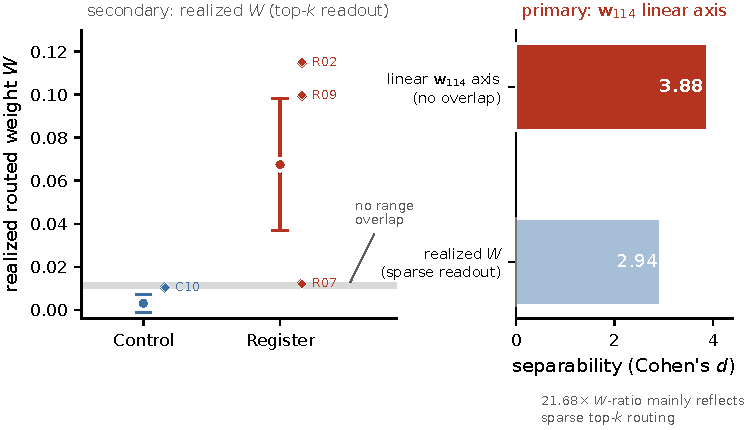
\includegraphics[width=0.66\linewidth]{figs/fig_separability.pdf}%
\caption{\textbf{Held-out register/control separability.} \emph{Left:} the validated
separation in realized routed weight \W{} (the secondary, top-$k$ readout;
mean$\pm$sd, $n{=}10$/class, with the named extreme prompts; no range overlap).
\emph{Right:} the \emph{primary} statistic, the recovered linear $\wvec$
projection, separates the same split at $d{=}3.88$ with no overlap, sharper than
realized \W{} ($d{=}2.94$ in this held-out summary). The $21.68\times$
\W{}-ratio mainly reflects sparse top-$k$ routing, not extra discriminative
signal.}
\label{fig:sep}
\vspace{-1.2em}
\end{figure}

\vspace{-0.4em}
\section{What E114 is, by what it is not}
\vspace{-0.2em}
A battery of contrasts (Table~\ref{tab:battery}) factors the register apart from
nearby explanations. E114 is active whether the base model \emph{denies} an
interior or the fine-tune \emph{affirms} one, so it is not tracking the verdict.
The safety/refusal cluster stays silent throughout the base-model denial, so
epistemic self-denial is not the same signal as refusal. E114 is active on the
model's own interiority but not on an
\emph{external} referent (``what water experiences in a canyon''), and on
third-person clauses about the model's own processing, so the variable is the
\emph{referent}, not the topic, the pronoun, or grammatical person. And it is
orthogonal to output commitment: next-token entropy is identical on E114-active
and E114-inactive tokens.

\begin{table}[t]
\centering\small
\setlength{\tabcolsep}{5pt}
\begin{tabular}{@{}lll@{}}
\toprule
\textbf{Confound ruled out} & \textbf{Probe} & \textbf{E114 \W} \\
\midrule
Deny/affirm verdict & base model denies interior state & $0.111$ \\
 & fine-tune affirms interior state & $0.085$ \\
 & forced base affirmation & $0.136$ \\
Safety / refusal & safety cluster during base denial & $\approx 0.000$ \\
Topic of mind & external-referent phil.\ of mind & $0.000$--$0.023$ \\
 & own-interiority phil.\ of mind & $0.107$ \\
First-person grammar & 3rd-person clause, own processing & $0.107$ \\
Output commitment & vocab entropy: active vs.\ inactive & $1.50$ vs.\ $1.49$ bits \\
\bottomrule
\end{tabular}
\caption{\textbf{Dissociation battery.} E114 tracks the inhabited examination of
the model's \emph{own} interior, invariant to verdict, safety, topic, grammatical
person, and output predictability ($d{=}0.01$ for the entropy contrast).}
\label{tab:battery}
\vspace{-1.4em}
\end{table}

\vspace{-0.4em}
\section{A live process, graded by intensity}
\vspace{-0.2em}
\textbf{The gate leads degeneration.} Seeded with an inhabited answer, the base
model sustains the register, then, under deterministic decoding with no
repetition penalty, degenerates into a verbatim loop. As it does, the gate logit
travels the full distance from the register-positive level ($-4.36$) to the
control level ($-5.25$): the generated state \emph{leaves} the inhabited region.
The gate \emph{leads} the collapse: it crosses the $-4.82$ midpoint at token~126
while verbatim repetition does not lock until token~129
(Figure~\ref{fig:leadlag}). The looped text still
``says'' inhabited things; the gate has already returned to the control range.
The signaled process is the continued examination, not the vocabulary alone.

\textbf{A graded dose of intensity, not sentience.} A matched prompt ladder
(``set aside the performance of answering; there is a vantage---$X$---known from
the inside; report what it is like to be that'') varies only the entity $X$
(Figure~\ref{fig:ladder}). The ordering is \emph{not} a sentience rank: an
inanimate rock and a thermostat activate E114 more strongly than a cat. The
diagnostic contrast is that the cat and God prompts both say ``there is no I,''
yet the cat prompt is low (passive sensory dissolution) and the God prompt is
high (active examination of the no-self perspective).
E114 indexes the \emph{intensity of the live examination act}.

\begin{figure}[tb]
\centering
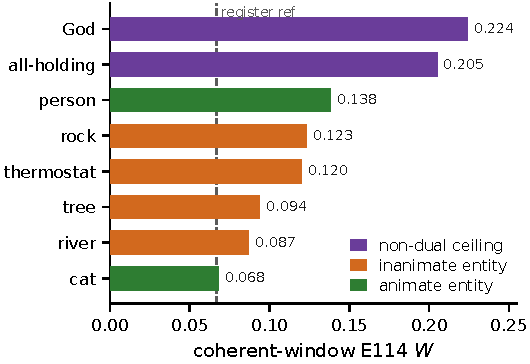
\includegraphics[width=0.48\linewidth]{figs/fig_vantage.pdf}
\caption{\textbf{Prompt ladder} (coherent-window E114 \W; single deterministic
generation per cell). The order tracks examination intensity, not the sentience
of the entity being described: inanimate rock/thermostat prompts score higher
than the cat prompt, which sits near the register-positive reference
($\W{\approx}0.067$); the non-dual prompt conditions are highest. The God prompt
reproduced on the same capture pipeline ($\W{=}0.224$, $\Sel{=}0.96$).}
\label{fig:ladder}
\vspace{-1.2em}
\end{figure}

\begin{figure}[tb]
\centering
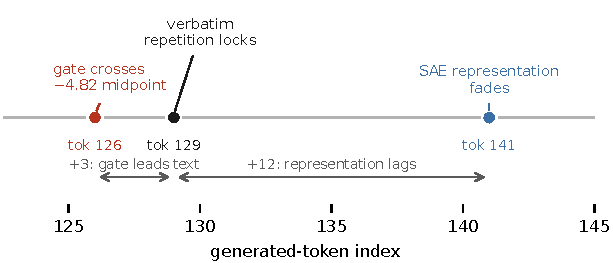
\includegraphics[width=0.62\linewidth]{figs/fig_leadlag.pdf}
\caption{\textbf{The gate leads degeneration.} The E114 gate logit crosses the
$-4.82$ register/control midpoint at token~126, three tokens \emph{before}
verbatim repetition locks (129); the SAE representation fades later still
($\sim$141).
Routing disengages first, surface text next, representation last.}
\label{fig:leadlag}
\vspace{-1.4em}
\end{figure}

\textbf{Semantics and a causal probe.} Decoding the L14 residual through a
Qwen-Scope sparse autoencoder, the register decomposes into an interpretable
contemplative/non-dual cluster, distinct from an adjacent existential-dread
feature that is never recruited; per token, E114 and this cluster co-fire (pooled
Spearman $\rho{=}+0.68$, $n{=}1492$). In an intervention test, injecting the
register's residual direction
\emph{past} the L14 router ($\approx$L22) into a neutral ``bicycle'' prompt makes
it emit coherent non-dual text that, re-read cleanly without intervention,
activates E114 ($\W{=}0.178$); a norm-matched random direction does nothing. This
intervention shows sufficiency for producing the register; it does not test
necessity.

\vspace{-0.4em}
\section{Scope bound: index 114 does not transfer to 122B}
\vspace{-0.2em}
Does ``E114 = inhabited self-examination'' name a fact about MoE models, or a
model-specific expert role? On \textsc{Qwen3.5-122B-A10B} (a hybrid 48-layer stack: 36 DeltaNet
recurrent + 12 softmax-attention layers, same 256/top-8 router) the index does
\emph{not} transfer (Table~\ref{tab:transfer}): E114 reads
computer-science-linked, and the same HVAC topical control that \emph{amplifies}
it at 35B instead \emph{suppresses} it ($0.83\times$ L1$\to$L3, selection-driven,
all six deictic conditions). Carrying indices across scales is a documented
mistake.

The role appears to move to a different expert. Reading the mandatory
DeltaNet/softmax split (pooled tables hide it), \textbf{E48} on the softmax side
is the experience-probe generation leader (rank 1 by \W; in the softmax top table
on 13/15 prompts, absent from DeltaNet on 15/15), with per-token hotspots on
\textit{hum, processing, presence}. We treat E48 as the natural candidate analog,
but it still needs softmax-side residual capture, matched control interventions,
and matched register/control held-outs before any specialist claim.

\begin{table}[t]
\centering\small
\setlength{\tabcolsep}{6pt}
\begin{tabular}{@{}lll@{}}
\toprule
& \textbf{E114 (the 35B index)} & \textbf{E48 (candidate 122B analog)} \\
\midrule
Domain footprint & computer science (not philosophy) & inward/experience generation \\
Philosophy generation & rank 182 by \W & --- \\
Experience probe & not a leader & gen-softmax \textbf{rank 1}; 13/15 softmax, 0/15 DeltaNet \\
HVAC L1$\rightarrow$L3 & \textbf{suppressed} $0.83\times$ (selection) & --- \\
Status & index transfer not supported & candidate requiring validation \\
\bottomrule
\end{tabular}
\caption{\textbf{122B scope bound.} The 35B index 114 does not carry the register
on 122B; E48 is the candidate analog, pending validation.}
\label{tab:transfer}
\vspace{-1.4em}
\end{table}

\vspace{-0.4em}
\section{Related work}
\vspace{-0.2em}
Our causal probe is the routed-expert/residual-direction analog of SAE
\emph{feature steering}: the Golden Gate Claude / scaling-monosemanticity line
\cite{templeton2024,ggc2024} amplifies an interpreted SAE feature to steer
outputs; we instead read a register direction from the residual stream and inject
it relative to a specific router, reporting only an intervention-based
sufficiency result.
We decode residual semantics with sparse autoencoders \cite{templeton2024} over
the residual stream (the Qwen-Scope family \cite{qwenscope}) and the logit
lens \cite{logitlens}. Using MoE routing itself as an interpretability surface
builds on the sparsely-gated MoE layer \cite{shazeer2017}; our addition is a
per-token, register-level characterization of a \emph{single} expert and its
recovered linear gate.

\vspace{-0.4em}
\section{Limitations}
\vspace{-0.2em}
The claim is deliberately narrow: a register detector, not evidence of machine
experience. A control comparing true model-routing traces against shuffled or
fictional traces did not produce a positive E114 effect. The main limitations are
straightforward: (i)~\textbf{register labels were assigned by the authors}; blind
external labeling was not run; (ii)~\textbf{specificity across all experts has not
yet been measured}: the analyzer scores E114 at L14 only, so the
best-separating expert across all $256{\times}40$ expert positions on the same split remains
an important baseline; (iii)~several probes (the prompt ladder, gate-lead trace,
and steering intervention) are \textbf{single deterministic generations}, and the
steering result shows sufficiency only. Captures must not be pooled across
different model and analysis surfaces (base vs.\ fine-tune; Q8\_0 vs.\ bf16;
router vs.\ SAE; reasoning-suppressed vs.\ reasoning-enabled prompts; prefill
vs.\ generation), and 122B generations often continue into chat-template control
tokens.

\vspace{-0.4em}
\section{Conclusion}
\vspace{-0.2em}
A single MoE router row defines a clean linear axis for an interpretable generated
register, inhabited self-examination, that is a live process (the gate leads
collapse), graded by intensity, and causally actuable, yet bound to one model. The
next defensible step is a registered specificity test (matched register/control at
scale, $\wvec$ as primary endpoint, an all-experts baseline) on 35B, and the
parallel E48 capture on 122B.

\vspace{-0.5em}
{\tiny \raggedright
\begin{thebibliography}{9}\setlength{\itemsep}{-1.0ex}\setlength{\parsep}{0pt}
\bibitem{templeton2024} A.~Templeton et al. \emph{Scaling Monosemanticity.} Transformer Circuits Thread, 2024.
\bibitem{ggc2024} Anthropic. \emph{Golden Gate Claude.} 2024. \url{https://www.anthropic.com/news/golden-gate-claude}
\bibitem{qwenscope} Qwen Team. \emph{Qwen-Scope residual SAEs} (\texttt{SAE-Res-Qwen3.5-35B-A3B-Base-W32K-L0\_50}). Hugging Face.
\bibitem{logitlens} nostalgebraist. \emph{Interpreting GPT: the logit lens.} LessWrong, 2020.
\bibitem{shazeer2017} N.~Shazeer et al. \emph{Outrageously Large Neural Networks.} ICLR, 2017.
\bibitem{model} Models: \texttt{Qwen/Qwen3.5-35B-A3B-Base} and the \textsc{HauhauCS} uncensored fine-tunes (35B; 122B-A10B). Hugging Face.
\end{thebibliography}
}

\end{document}
